\chapter{Structure Method}
In this section the waterfall and iterative methods, both used to structure a project, will be described. The concepts of the methods, strengths and weaknesses will be discussed. This information will then be used to support the choice of method. Afterwards the chosen method and its application in the documentation will be described.

The waterfall is a sequential method with a progressive project process, which avoids revision of the finished parts. This means that a part is worked upon until it satisfies certain requirements, and then the project members move on to the next part. The iterative method focuses on multiple iterations of the project process and therefore iterating through the project multiple times, expanding the product and documentation each time.

Both methods have their strengths and weaknesses and one method might have a strength that is a weakness for the other. One of the strengths of the waterfall method is the consecutive order of progress the structure gives. This gives the project members an overview of how far they are in a specific part or in the overall progress of the project. This overview is obtained as the project members can document when a part of the project is finished. Another strength of this method is the ease of setting deadlines for the parts in the documentation and using these deadlines to measure the progress of the project. The consecutive nature of the method can also become a weakness. During the project, information can change and this can result in previous parts of the documentation not including or reflecting on the new information. This leads to another weakness of whether or not the product of the project really is complete when the project is completed? The project can expand and new information can change, add or subtract requirements for the final product, making it difficult to conclude that the product is complete when the project is done. 

The iterative method has the strength that it is dynamic. Each iteration of the project process allows the addition of new information and changes. When using this method it can be difficult to keep an overview because each iteration adds more information. On the other hand each iteration gives a better understanding of the project context, development and requirements. This could lead to an endless circle of improving and expanding the project, rendering it difficult to say when the project is actually finished. This could prove to be difficult to answer, whereas the waterfall method gives a structure that restricts the multiple iterations and sets an end point. 

The waterfall method provides an easy overview of the project progress. It is also a good choice because the system requirements and the goals that have been set, can be defined after each part of the documentation. This allows for confirmation on the goals and requirements that have been set. The waterfall method will therefore be used in this project.       

When documenting a project using the waterfall method as a structure, it is necessary to write five different parts which covers the project process from start to finish.

\textbf{The analysis part} focuses on getting to know the project in context e.g. to the audience or the environment. This part is referred to as \textit{\nameref{part:ProbAnal}} in the report. It is based on relevant sources e.g. articles, documentations, questionnaires or interviews which satisfies a certain standard of source criticism and relevance. In this project the information is gathered through external sources and interviews. The information is then used to define a problem statement for the following parts of the report and solution.

\textbf{The design part} is used to identify design specifications that is needed in a certain product. In our report, the design part focuses on the principles learned in the courses \textit{Design and Evaluation of User Interfaces} and \textit{Object Oriented Analysis and Design} (OOAD). In this part of the report, the interface design is modeled by using scenario-based design. The architectural design is created by using OOAD techniques. 

\textbf{The implementation part} is the part in which the software is created. The design specifications are used to make the design, and the needed functionality requirements which were identified throughout the analysis part is implemented. The outcome of this process in the project is a functional program.

\textbf{The system test part} is used for validating the system to ensure that it satisfies the stated requirements and goals regarding both usability and quality. The system is tested to secure that it is of high quality and the usability of the program is tested as well. The outcome of this process is a test part documented in the report.

\textbf{The system in operation} concerns the system after it is published. The report incorporates a reflection part which suggests future improvements.

\begin{figure}[H]
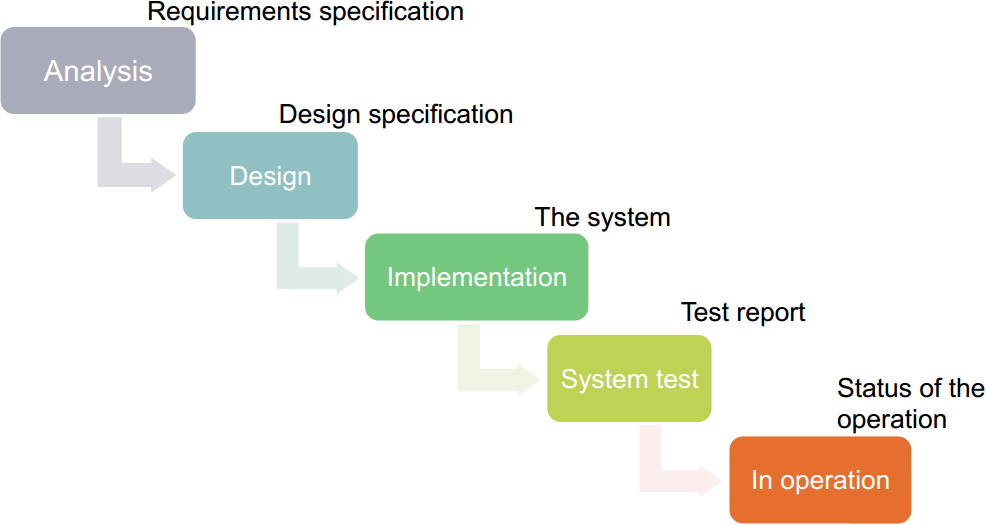
\includegraphics[width=\linewidth, clip=true]{Grafik/FoodPlanner/Waterfall}
\centering
\caption{Model representing the waterfall method}
\end{figure}